\documentclass[11pt,a4paper,openany,leqno]{article}

\textwidth=160mm \textheight=260mm \hoffset=-18mm \voffset=-30mm
\setcounter{page}{1}
			\usepackage[magyar]{babel}
			\usepackage[utf8]{inputenc}
			\usepackage[T1]{fontenc}
			\usepackage{indentfirst}
			\usepackage{amsmath,esint}
			\usepackage{amssymb}
%			\usepackage{eufrak}
			\usepackage{psfrag}
			\usepackage{tabularx}
			\usepackage{graphicx}
			\usepackage{wrapfig}	
			\usepackage{hyperref}
			\usepackage{multicol}	
									
			\frenchspacing
			\allowhyphens

\tolerance=2000
\hbadness=2000
\vbadness=10000
\overfullrule=0pt




\begin{document}
\section{Elektromágneses hullálok}
\subsection{Kovács-Párkányi Fizikai Példatár II. / 251. feladat}
Milyen vastagságú folyadékreteget kell egy üveglap felületére helyezni, hogy ez a felület $\lambda = 5000 $ Å hullámhosszúságú fény számára merőleges beesés esetén nem reflektáló felület legyen? Az üveg abszolút törésmutatója $1,52$, a folyadéké $1,3$.
\begin{figure}[h!]
\centering
  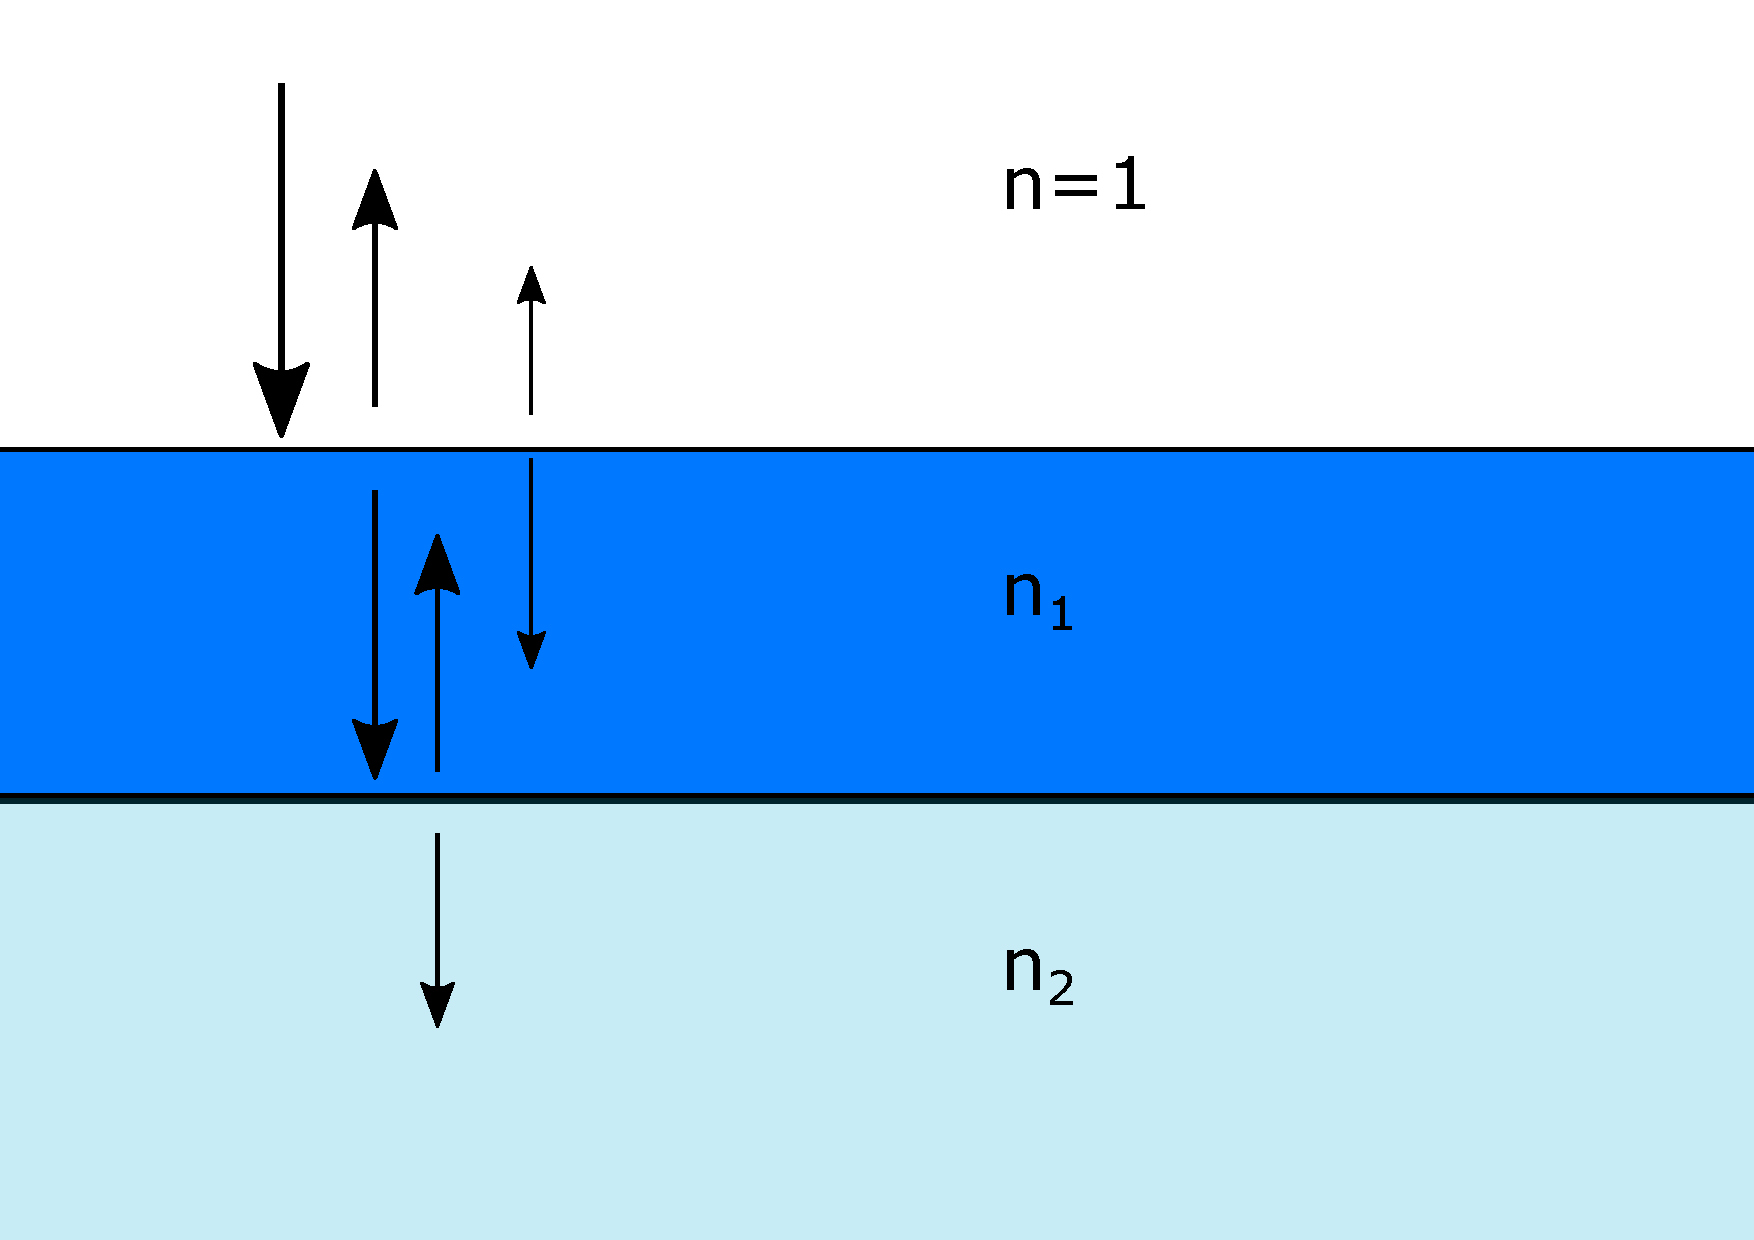
\includegraphics[width=120mm,scale=0.5]{kep.pdf}
  \caption{A hosszú egyenes vezető és a gyűrű}
  \label{}
\end{figure} 
 \indent





\begin{flushright} {Feladatot kidolgozta: {\it Z2R8XS}} \end{flushright}

\vspace{0.5cm}

\textbf{Megoldás}\\
\indent
A relatív törésmutató az egy-egy közegben való terjedés között képvisel összefüggést, a megtörésről is tartalmaz információt. A törésmutató egy dimenziótlan szám, mely egyes mennyiségek arányára utal.\\
\indent A beesési szög és a kilépési szög színuszának arányát. A Snellius-Descartes törvényből kijön, hogy a merőlegesen beeső fény trajektóriája nem változik.\\
\indent A fény első közegben való terjedési sebessége és a második közegbeli sebességének aránya.\\

\indent
A törésmutató, ha az $1$-es közegből a $2$-es közegbe kerül a fény.\\
$$ n_{21} = \frac{c_1}{c_2} $$
\indent
A terjedési sebesség, a hullámhossz és a frekvencia között fennáll a $c = \lambda \cdot f$ összefüggés. A frekvencia a törés során nem változik. Ezek szerint, ha a terjedési sebesség változik, a hullámhossznak is muszáj változnia.\\
$$ n_{21} = \frac{c_1}{c_2} = \frac{\lambda_1 \cdot f}{\lambda_2 \cdot f} = \frac{\lambda_1}{\lambda_2} $$\indent
Nem reflektáló felület létrehozásához az kell, hogy a beeső fény kioltsa a visszavert fény egy részét, a többi rész pedig vagy elnyelődjön, vagy tovább haladjon. Elnyelődésről nem beszél a feladat, így a másik két szempont szerint kell eljárni.\\ \indent
A fénysugár egy része a vákuum és a folyadék határán visszaverődik, egy része behatol a folyadékba. A Maxwell egyenletek azt mondják, hogy az elektromos tér közeghatárral párhuzamos komponense folytonosan megy át - a merőleges beesés miatt itt csak párhuzamos komponens van. A törésmutatóktól függ, hanyad rész transzmittálódik, illetve reflektálódik. A visszavert fény kap egy $\pi$ relatív fázist a beeső fényhez képest. \\ \indent
A folyadékba behatoló fénysugár egy része a folyadék és az üveglap határán visszaverődik, egy része behatol az üveglapba. Vegyük úgy, hogy az üveglapba behatolt fény már nem fog visszatérni. Az itt visszavert fény úgyszint egy $\pi$ relatív fázist fog kapni. A folyadékban előforduló hullámhossz a fenti módon kiszámolható.\\ \indent
A folyadék és az üveg határáról visszavert fény egy része a vákuum és a folyadék határára érve újra visszaverődik, egy része kijut a folyadékból. A fény egy része mindig "pattogni" fog a két határfelület között. Amint a fény bármilyen közegben halad, változik a fázisa (a megtett út és a hullámszám vektor hosszának szorzata adja meg ezt a változást). A folyadék felszínére visszaérő fény fázisa függ attól, mennyi utat tett meg a fény a folyadékban. A merőleges beesés miatt a fény mindig a folyadékréteg vastagságának megfelelő távolság egész számú többszörösét fogja megtenni.\\
\indent
Azt szeretnénk, hogy a folyadék és az üveg határáról visszaverődött fény destruktív interferenciát szenvedne. Ez úgy érhető el, ha a folyadékba behatoló és a folyadékból kilépő fénysugarak fázikülönbsége $\pi$ legyen - pontosabban $(2N+1) \cdot \pi$, ahol $N$ egy terméeszetes szám. Legyen $\lambda_1$ a folyadékbeli hullámhossz.\\
$$ 2kd + \pi = (2N+1) \cdot \pi $$
$$ 2\frac{2\pi}{\lambda_1}d + \pi = (2N+1) \cdot \pi $$
$$ 2\frac{2\pi}{\lambda_1}d = 2N \cdot \pi $$
$$ \frac{2}{\lambda_1}d = N $$
$$ 2d = N\lambda_1 $$
$$ 2nd = N\lambda $$
Ahol $\lambda$ az eredeti hullámhossz. Tehát a folyadék vastagságának a fél hullámhossz egész többszörösének kell lennie.






\end{document}